\documentclass[10pt]{article}
\usepackage[letterpaper,margin=0.75in]{geometry}
\usepackage{graphicx}
\usepackage{booktabs}
\usepackage{amsmath}
\usepackage{xcolor}
\usepackage{listings}
\usepackage{enumitem}
\usepackage[hidelinks]{hyperref}
\usepackage{caption}
\usepackage{float}
\captionsetup{font=small,labelfont=bf}
\setlist{nosep,leftmargin=1.4em}
\setlength{\parskip}{3pt}
\setlength{\parindent}{0pt}
\lstset{basicstyle=\ttfamily\footnotesize,columns=fullflexible,frame=single,framerule=0.3pt,
        rulecolor=\color{gray!60},xleftmargin=2pt,xrightmargin=2pt,aboveskip=4pt,belowskip=2pt}
\newcommand{\code}[1]{\texttt{#1}}

\title{\vspace{-1.6em}\textbf{Fast Direct Convolution for YOLOv8n on Broadwell}\\[2pt]
\large Mid-project design document: the 3$\times$3 stride-1 kernel}
\author{Om Tank \quad (team: Om Tank, O'Malley Sherlock, Bohan (Simon) Yu)\\
18-645 How to Write Fast Code I, Fall 2026}
\date{\vspace{-1.2em}}

\begin{document}
\maketitle

\noindent Our project writes FP32 direct-convolution kernels for the pretrained YOLOv8n detector and compares them with OpenCV DNN and ONNX Runtime on the same ONNX model and images. YOLOv8n has three kinds of convolution; I own the 3$\times$3, stride-1, pad-1 kernel. It covers 32 of the 64 conv layers (the two convs in every C2f bottleneck plus the first two convs of each Detect branch) and 5.80 of the 8.74 GFLOP per 640$\times$640 image (66\%). All numbers below were measured on ece028, single core, batch 1, unless stated otherwise. Every version is checked against the baseline model's own outputs on real images (max relative error $\le 10^{-4}$; measured $\le 2.6\times10^{-5}$).

\section{Kernel description}
For each image $n$, output channel $k$ and output pixel $(h,w)$:
\[ y_{n,k,h,w} = \mathrm{SiLU}\Big(b_k + \textstyle\sum_{c=0}^{C-1}\sum_{r=0}^{2}\sum_{s=0}^{2} x_{n,c,h+r-1,w+s-1}\, W_{k,c,r,s}\Big). \]
\begin{itemize}
\item \textbf{Independent operations.} Every output element is an independent dot product of length $9C$. A layer has $K\cdot H\cdot W$ of them, between 25{,}600 and 512{,}000 for our layers, far more than the machine needs.
\item \textbf{Dependent instructions.} Inside one output, the reduction is a chain of $9C$ fused multiply-adds into one accumulator, each depending on the previous one (144 to 2{,}304 FMAs long). With SIMD, 8 output channels share one chain in one register.
\item \textbf{Functional units.} FMA units on ports 0 and 1; loads (weights and broadcast inputs) on ports 2 and 3; one store per output vector on port 4. The SiLU epilogue uses the FMA/multiply units and the divider.
\item \textbf{SIMD.} AVX2 with FMA3: 16 YMM registers of 8 FP32 lanes (\code{vfmadd231ps}, \code{vbroadcastss}).
\item \textbf{Specialized units.} None for FP32 on this CPU: no AVX-512, no VNNI or AMX (those target int8/bf16 anyway); F16C only converts half precision. BatchNorm is not a kernel: the ONNX export already folds it into $W$ and $b$, so it costs nothing at inference.
\end{itemize}

\section{Performance peak}
\textbf{Machine.} ece028: Intel Xeon E5-2640 v4 (Broadwell-EP), 2 sockets $\times$ 10 cores (Hyper-Threading, 40 threads, 2 NUMA nodes), 2.4\,GHz base; a single busy core measured 3.39\,GHz (turbo). 32\,KB L1D and 256\,KB L2 per core, 25\,MB L3 per socket. GCC 8.5.0 (Red Hat 8.5.0-28), \code{-O3 -march=broadwell -mtune=broadwell -fopenmp}. Cycles are read from the core cycle counter (\code{perf\_event}), so turbo does not distort FLOPs/cycle.

\begin{table}[H]\centering\small
\begin{tabular}{lllll}
\toprule
Instruction & Role & Latency & Throughput & Ports\\
\midrule
\code{vfmadd231ps ymm} & 8-lane multiply-add & 5 cycles & 2 / cycle & 0, 1\\
\code{vbroadcastss ymm,m32} & 1 input to 8 lanes & $\approx$5--6 & 2 / cycle & 2, 3\\
\code{vmovaps ymm,m256} & 8 weights & $\approx$5--6 & 2 / cycle & 2, 3\\
\code{vmovaps m256,ymm} & output store & -- & 1 / cycle & 4\\
\bottomrule
\end{tabular}
\caption{Instructions of the kernel (Broadwell). The FMA numbers match our Assignment 1 measurements; v1 below re-measures the latency directly.}
\end{table}

\textbf{Theoretical peak.} Per core: 2 FMA/cycle $\times$ 8 lanes $\times$ 2 FLOPs = \textbf{32 FLOPs/cycle}; 640 FLOPs/cycle for 20 cores (1{,}536 GFLOP/s at the 2.4\,GHz base). The kernel is FMAs plus a short epilogue per output vector (bias is free, it initializes the accumulator; SiLU is about 20 vector operations against $9C\ge144$ FMAs), so the kernel's peak is essentially the machine's: measured, turning SiLU off on the $C=64$ layer gains under 1\% (25.66 vs 25.89 FLOPs/cycle). Reaching it needs two things: at least latency $\times$ throughput $= 5 \times 2 = 10$ independent accumulators in flight, and few enough loads per FMA that the 2 load ports keep up.

\section{Design and implementation}
\textbf{Data layout} (detailed in Section~\ref{sec:mem}): activations are NCHW8c with a 1-pixel zero halo, so the 8 channels of a pixel are one aligned 32-byte load and the 3$\times$3 window never needs an edge test; weights are packed so the 8 output-channel weights of one (input channel, tap) are one aligned load.

\textbf{Register tile.} One microkernel call computes $K_B$ output-channel blocks of 8 $\times$ $O_W$ consecutive output pixels of one row. Each inner step (one input channel, one tap) loads $K_B$ weight vectors, broadcasts $O_W$ input values, and issues $K_B O_W$ FMAs (every weight meets every input).
\begin{table}[H]\centering\small
\begin{tabular}{cccccl}
\toprule
Tile & Acc. & YMM & Loads/step & FMAs/step & Verdict\\
\midrule
1$\times$10 & 10 & 12 & 11 & 10 & load-bound (11 loads $>$ 10 slots in 5 cycles)\\
\textbf{2$\times$5} & \textbf{10} & \textbf{13} & \textbf{7} & \textbf{10} & \textbf{chosen: divides every width and every $K/8$}\\
2$\times$6 & 12 & 15 & 8 & 12 & no width divides by 6; needs row tails (tried as v4)\\
3$\times$4 & 12 & 16 & 7 & 12 & $K/8 \in \{2,4,8,10,16\}$ is never divisible by 3\\
4$\times$3 & 12 & 17 & 7 & 12 & does not fit in 16 registers\\
\bottomrule
\end{tabular}
\caption{Tile candidates.}
\end{table}

\begin{enumerate}[label=(\alph*)]
\item \textbf{Size.} 2 blocks $\times$ 8 channels $\times$ 5 pixels = \textbf{80 outputs} per call, each fully reduced over $9C$ inputs before it is stored.
\item \textbf{Registers.} 13 needed of the 16 YMM available: 10 accumulators, 2 weights, 1 broadcast. The generated assembly has no stack spills in the FMA loop.
\item \textbf{Allocation.} \code{acc[0][0..4]} = outputs of block $k_b$ at pixels $w..w{+}4$; \code{acc[1][0..4]} = block $k_b{+}1$; \code{wv[0]}, \code{wv[1]} = the 8 weights of each block for the current (input channel, tap); \code{x} = the current input value broadcast to 8 lanes.
\item \textbf{Reuse.} Each weight register feeds 5 FMAs (one per pixel); each broadcast feeds 2 (one per block); accumulators stay in registers for the whole reduction and are written to memory once; the bias is loaded once as the accumulators' initial value.
\item \textbf{Implementation.} \code{ukr<KB,OW>} is a C++ template so both inner loops fully unroll and every accumulator gets its own register; the input-channel loop is unrolled 8$\times$. The driver walks $(n,\ k_b\text{ pair},\ h,\ w\text{ step } 5)$; v3 adds OpenMP over the first three loops.
\end{enumerate}
\begin{lstlisting}
acc[k][j] = bias[kb+k]                         for k < 2, j < 5      // 10 YMM
for cb in 0 .. C/8-1:                           // input-channel block
  for r, s in 0..2 x 0..2:                      // tap of the 3x3 window
    for ci in 0..7:                             // channel inside the block (unrolled)
      wv[k] = load W[kb+k][cb][r][s][ci][0..7]       for k < 2     // 2 loads
      for j in 0..4:
        x = broadcast X[cb][h+r][w+j+s][ci]                       // 5 broadcasts
        acc[k][j] = fma(x, wv[k], acc[k][j])         for k < 2     // 10 FMAs
store SiLU(acc[k][j]) to Y[kb+k][h][w+j][0..7]
\end{lstlisting}

\textbf{Measured staircase} (Figure~\ref{fig:stair}). Each version removes one bottleneck. The textbook loop (\code{ref}) runs at 0.29 FLOPs/cycle. v0 is the same scalar code on the blocked layout: with 8 channels contiguous the compiler vectorizes the innermost loop itself (as separate multiply and add), giving 2.84. v1 writes the 8-wide FMA explicitly but keeps one accumulator: it measures \textbf{3.23 FLOPs/cycle on every layer, exactly $32/10$}, i.e.\ one 16-FLOP FMA per 5-cycle latency. v2 (2$\times$5) hides the latency: \textbf{24.68 FLOPs/cycle, 77\% of peak} over all 32 layers (21.3--25.8 per layer).

\begin{figure}[H]\centering
\begin{minipage}{0.53\linewidth}\centering
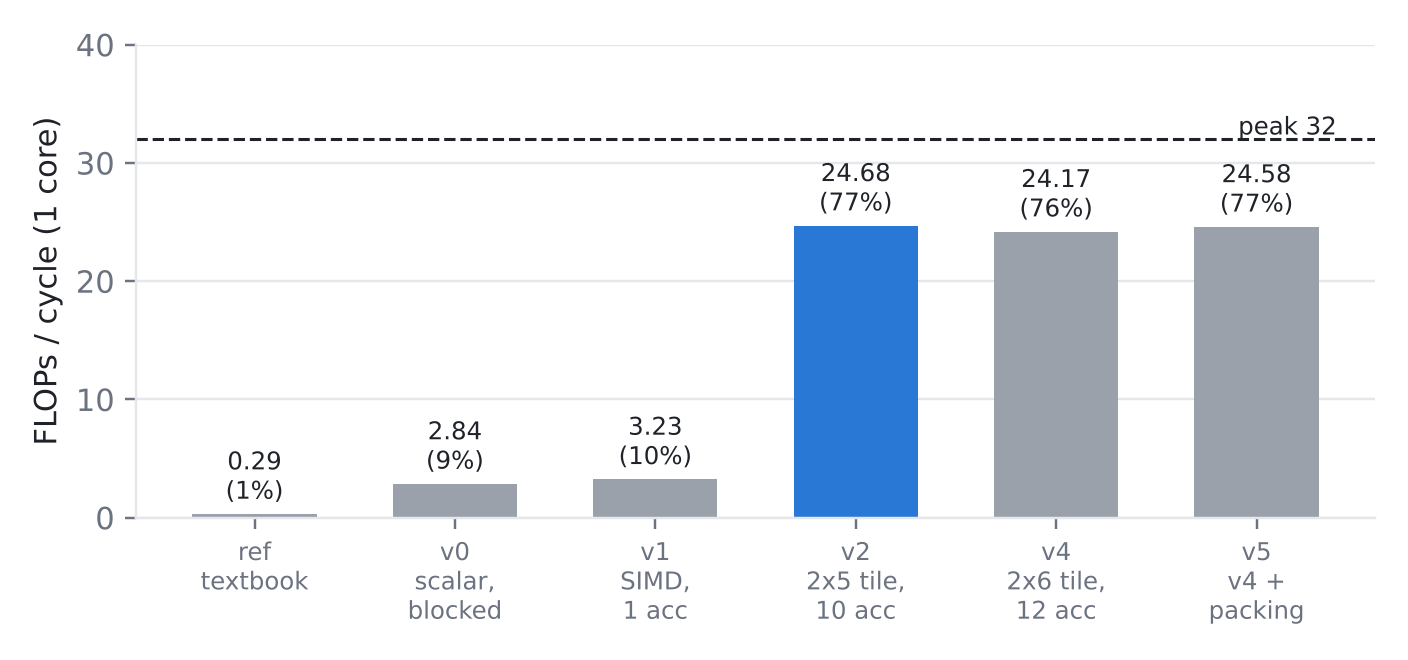
\includegraphics[width=\linewidth]{figs/staircase.png}
\caption{FLOPs/cycle over all 32 layers, one core.}\label{fig:stair}
\end{minipage}\hfill
\begin{minipage}{0.45\linewidth}\centering
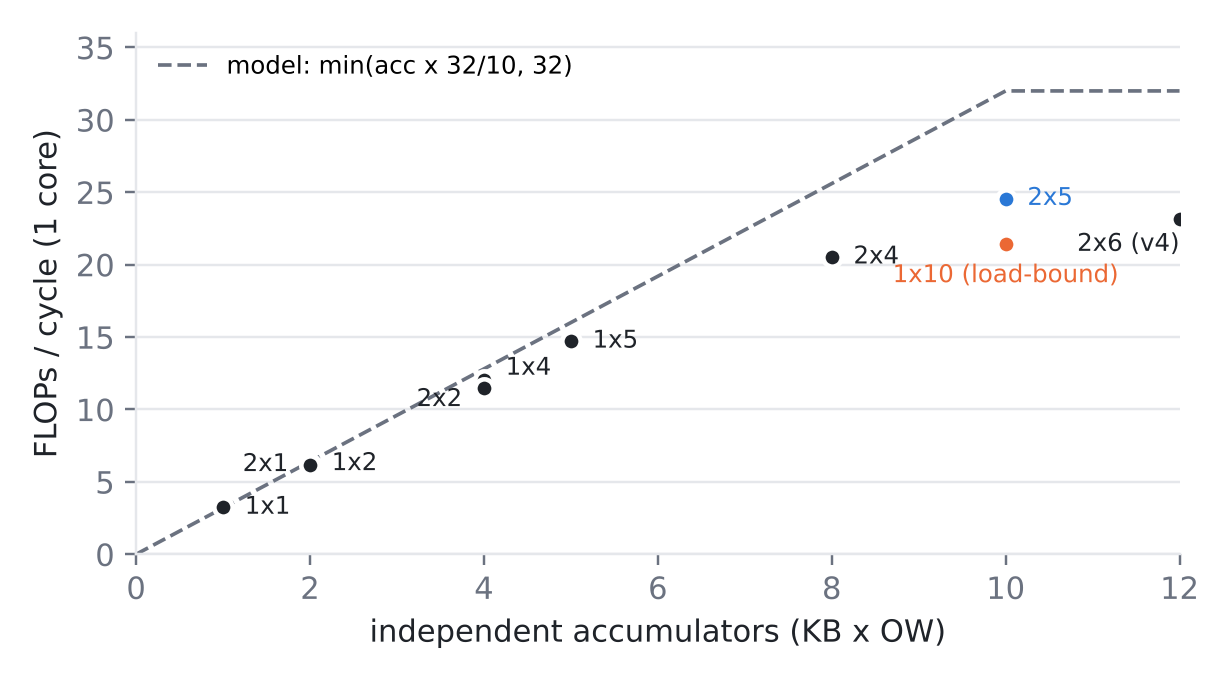
\includegraphics[width=\linewidth]{figs/accumulators.png}
\caption{Same microkernel, different tiles (mean of $C$=16, 32, 64, 128 layers).}\label{fig:acc}
\end{minipage}
\end{figure}

\textbf{Accumulator experiment} (Figure~\ref{fig:acc}). Throughput rises by $\approx$3.2 FLOPs/cycle per accumulator and reaches 90--101\% of the latency model up to 5 accumulators, then bends: 80\% of the model at 8 and 77\% at 10. 1$\times$10 has the same 10 accumulators as 2$\times$5 but 11 loads per 10 FMAs and drops to 21.4, the register-reuse argument measured.

\textbf{Where the last 23\% goes.} Hardware counters on the $C=64$ layer (v2, 1{,}000 runs): 2.95 uops issued per cycle (limit 4), so the front end is not the limit; ports 0 and 1 are each busy 80--81\% of cycles and run almost only FMAs (7.75\,G uops for 7.39\,G FMAs), so no other instruction steals FMA slots; but allocation is stalled in 24\% of cycles, half of it on a full scheduler (RS), none on the ROB or store buffer. The core issues faster than two FMA units retire, the scheduler fills with FMAs waiting on their running sums, and the broadcast loads of the next steps cannot enter early, so their latency shows. This also explains the two follow-ups that did \emph{not} help: \textbf{v4} (2$\times$6, 12 accumulators, 6+2 or 4+4 row tails) reaches 24.17--24.49, and \textbf{v5} (v4 plus weights repacked into the exact reading order, one contiguous stream) 24.58: extra slack on the FMA side does not help when the stall is on the load side. The fix is explicit software pipelining (issue loads one step ahead), which compilers do not schedule reliably and BLIS does in inline assembly; that is our next step.

\textbf{Multi-core.} v3 on 20 threads (one per physical core) runs all 32 layers in 5.09\,ms vs 69.5\,ms on one core (13.7$\times$), 1{,}140 GFLOP/s, 74\% of the 20-core peak at the 2.4\,GHz base clock. Thread pinning, NUMA first-touch and batch $>1$ are not yet tuned.

\section{Memory hierarchy design}\label{sec:mem}
An intermediate layout \emph{is} required; the plain NCHW/OIHW layouts of ONNX give the microkernel neither contiguous 8-channel vectors nor branch-free borders.
\begin{itemize}
\item \textbf{Activations: NCHW8c with a halo,} stored \code{[N][C/8][H+2][W+2][8]}. The 8 innermost floats are 8 consecutive channels, one register; the 5 pixels a call needs are 32 bytes apart in the same cache lines. The zero border stores the padding explicitly, so every call is identical. A kernel writes only the interior of its output, so the next layer can read it directly.
\item \textbf{Weights:} packed offline (like BatchNorm folding) to \code{[K/8][C/8][3][3][8 in][8 out]}; v5 interleaves the two output blocks of a tile, \code{[K/16][C/8][3][3][8 in][2][8 out]}, so the microkernel reads one stream in order.
\item \textbf{One layout for the whole network.} The whole team codes against this one contract (\code{include/common.h}); the stride-2 and 1$\times$1 kernels use it too, so layers chain with no conversion. In NCHW8c each 8-channel block is its own plane, so the C2f \emph{Split} is a pointer offset and \emph{Concat} is the producer writing into its slice of a larger buffer, both free. The only conversions are at the network input and output.
\item \textbf{Working set.} Per tile pair the weight slab is $576C$ bytes: 9, 18, 37, 74 and 147\,KB for $C$ = 16, 32, 64, 128, 256 against a 32\,KB L1 and 256\,KB L2. It is reused across a whole output plane, so even L2-resident slabs keep 73--80\%; only the two $C=256$ head layers (67--71\%), whose weights and 400\,KB input both exceed L2, lose noticeably. Blocking the input-channel loop (or a Morton-ordered traversal of output tiles) for those layers is future work.
\end{itemize}

\section{Performance baseline}
Both baselines run the same ONNX model on the same images, single-threaded, timed per layer (OpenCV DNN \code{getPerfProfile}, ONNX Runtime profiler). Their FLOPs/cycle use the measured 3.39\,GHz core clock so all three are in real cycles. Data type: FP32 only; sizes: the 11 distinct layer shapes (Figure~\ref{fig:base}).
\begin{figure}[H]\centering
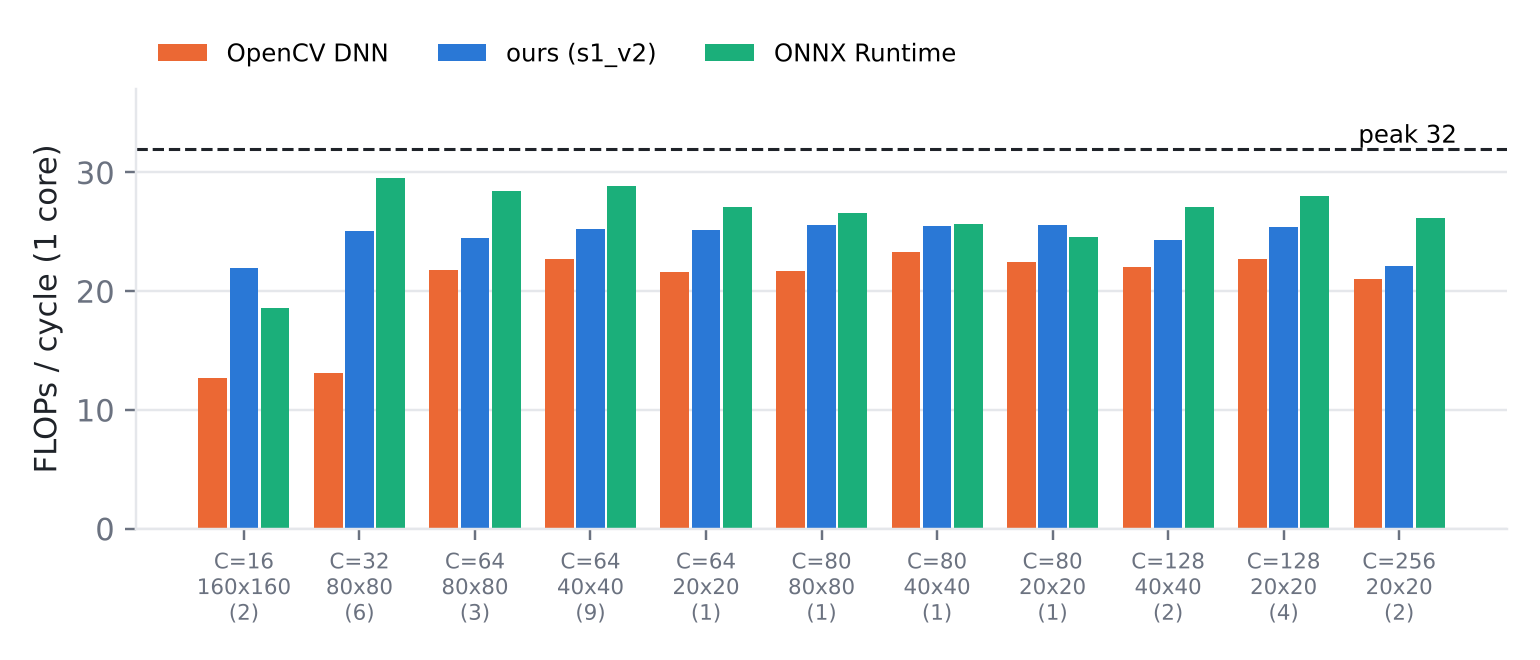
\includegraphics[width=0.86\linewidth]{figs/layers_vs_baselines.png}
\caption{FLOPs/cycle per layer shape (number of layers in parentheses), one core. Dashed line: 32 FLOPs/cycle peak.}\label{fig:base}
\end{figure}
\begin{itemize}
\item \textbf{Baselines vs peak.} OpenCV DNN: 19.8 FLOPs/cycle overall (\textbf{62\%} of peak), 12.7--23.3 per layer, weakest on the $C\le32$ layers (about 40\%). ONNX Runtime: 27.4 (\textbf{86\%}), 18.6--29.7 per layer.
\item \textbf{Ours vs peak.} 24.7 (\textbf{77\%}), 21.3--25.8 per layer, and more uniform across shapes than either baseline: on the $C=16$, 160$\times$160 layers we reach 69\% where ONNX Runtime reaches 58\% and OpenCV 40\%. Total time for the 32 layers: 69.5\,ms (ours), 86.4\,ms (OpenCV DNN), 62.6\,ms (ONNX Runtime).
\end{itemize}
Next steps: software-pipelined (hand-scheduled) microkernel for the last $\approx$20\%, cache blocking for the $C=256$ layers, NUMA-aware threading, and batch 16.

\end{document}
